\begin{comment}
\chapter{Time complexity}
\end{comment}
\chapter{時間計算量}

\index{time complexity}
\index{時間計算量}

\begin{comment}
The efficiency of algorithms is important in competitive programming.
Usually, it is easy to design an algorithm
that solves the problem slowly,
but the real challenge is to invent a
fast algorithm.
If the algorithm is too slow, it will get only
partial points or no points at all.

The \key{time complexity} of an algorithm
estimates how much time the algorithm will use
for some input.
The idea is to represent the efficiency
as a function whose parameter is the size of the input.
By calculating the time complexity,
we can find out whether the algorithm is fast enough
without implementing it.
\end{comment}

競技プログラミングにおいてアルゴリズムの効率は重要である。
一般的に、遅いアルゴリズムの設計は簡単であるが、高速なアルゴリズムの発明は
難しいチャレンジと言える。
もしアルゴリズムが遅すぎれば、コンテストでは0点かせいぜい部分点しか得られない。

アルゴリズムの時間計算量(\key{time complexity})は、入力に対し
どの程度の時間がかかるかを概算するための概念である。
時間計算量のアイデアは、入力長をパラメータとする関数で実行時間を表すものである。
この時間計算量を算出することで、アルゴリズムに対し実際に実装することなく
十分に高速かどうか予測できる。


\begin{comment}
\section{Calculation rules}

The time complexity of an algorithm
is denoted $O(\cdots)$
where the three dots represent some
function.
Usually, the variable $n$ denotes
the input size.
For example, if the input is an array of numbers,
$n$ will be the size of the array,
and if the input is a string,
$n$ will be the length of the string.
\end{comment}

\section{計算手順}

アルゴリズムの時間計算量は$O(\cdots)$と表記される(3点ドットは何らかの関数である)。
通常、変数$n$で入力長を表す。
例えば入力が整数列の場合$n$は数列の要素数であり、入力が文字列ならば$n$は文字列長である。

\begin{comment}
\subsubsection*{Loops}

A common reason why an algorithm is slow is
that it contains many loops that go through the input.
The more nested loops the algorithm contains,
the slower it is.
If there are $k$ nested loops,
the time complexity is $O(n^k)$.

For example, the time complexity of the following code is $O(n)$:
\end{comment}

\subsubsection*{ループ}

アルゴリズムが遅い一般的な理由はループが深いことにある。
深い多重ループを含むアルゴリズムほど遅くなる。
もしアルゴリズムが$k$重ループを含むとき、その時間計算量は$O(n^k)$と表記される。

例えば、以下の一重ループの時間計算量は$O(n)$である:

\begin{lstlisting}
for (int i = 1; i <= n; i++) {
    // code
}
\end{lstlisting}

\begin{comment}
And the time complexity of the following code is $O(n^2)$:
\end{comment}
以下の二重ループでは時間計算量は$O(n^2)$となる:

\begin{lstlisting}
for (int i = 1; i <= n; i++) {
    for (int j = 1; j <= n; j++) {
        // code
    }
}
\end{lstlisting}

\begin{comment}
\subsubsection*{Order of magnitude}

A time complexity does not tell us the exact number
of times the code inside a loop is executed,
but it only shows the order of magnitude.
In the following examples, the code inside the loop
is executed $3n$, $n+5$ and $\lceil n/2 \rceil$ times,
but the time complexity of each code is $O(n)$.
\end{comment}

時間計算量の表記は、ループの正確な回数を示すものではなく、大よそのオーダーを示すものに過ぎない。
下記のコードのループ回数はそれぞれ$3n$, $n+5$, $\lceil n/2 \rceil$回だが、
いずれも時間計算量は$O(n)$と表現される。

\begin{lstlisting}
for (int i = 1; i <= 3*n; i++) {
    // code
}
\end{lstlisting}

\begin{lstlisting}
for (int i = 1; i <= n+5; i++) {
    // code
}
\end{lstlisting}

\begin{lstlisting}
for (int i = 1; i <= n; i += 2) {
    // code
}
\end{lstlisting}

\begin{comment}
As another example,
the time complexity of the following code is $O(n^2)$:
\end{comment}

別の例として、以下のコードの時間計算量は$O(n^2)$である:

\begin{lstlisting}
for (int i = 1; i <= n; i++) {
    for (int j = i+1; j <= n; j++) {
        // code
    }
}
\end{lstlisting}

\begin{comment}
\subsubsection*{Phases}

If the algorithm consists of consecutive phases,
the total time complexity is the largest
time complexity of a single phase.
The reason for this is that the slowest
phase is usually the bottleneck of the code.

For example, the following code consists
of three phases with time complexities
$O(n)$, $O(n^2)$ and $O(n)$.
Thus, the total time complexity is $O(n^2)$.
\end{comment}

\subsubsection*{手順}

もしアルゴリズムがいくつかの手順を踏む場合、全体の時間計算量は
ここの手順の最大値となる。
その理由は、最も大きな時間計算量の手順が通常コードのボトルネックと
なるためである。

例えば以下のコードは3つの手順からなり、
それぞれの時間計算量は$O(n)$, $O(n^2)$, $O(n)$である。
よって全体の時間計算量は$O(n^2)$となる.

\begin{lstlisting}
for (int i = 1; i <= n; i++) {
    // code
}
for (int i = 1; i <= n; i++) {
    for (int j = 1; j <= n; j++) {
        // code
    }
}
for (int i = 1; i <= n; i++) {
    // code
}
\end{lstlisting}

\begin{comment}
\subsubsection*{Several variables}

Sometimes the time complexity depends on
several factors.
In this case, the time complexity formula
contains several variables.

For example, the time complexity of the
following code is $O(nm)$:
\end{comment}

\subsubsection*{複数変数がある場合}

時間計算量は複数パラメータに依存することもある。
この場合、時間計算量の式も複数の変数を含む。

例えば以下のコードの時間計算量は$O(nm)$である:

\begin{lstlisting}
for (int i = 1; i <= n; i++) {
    for (int j = 1; j <= m; j++) {
        // code
    }
}
\end{lstlisting}

\begin{comment}
\subsubsection*{Recursion}

The time complexity of a recursive function
depends on the number of times the function is called
and the time complexity of a single call.
The total time complexity is the product of
these values.

For example, consider the following function:
\end{comment}

\subsubsection*{再帰}

再帰関数の時間計算量は、関数の実行回数と1回の実行あたりの時間計算量の積となる。

例えば以下の関数を考えてみる:

\begin{lstlisting}
void f(int n) {
    if (n == 1) return;
    f(n-1);
}
\end{lstlisting}

\begin{comment}
The call $\texttt{f}(n)$ causes $n$ function calls,
and the time complexity of each call is $O(1)$.
Thus, the total time complexity is $O(n)$.

As another example, consider the following function:
\end{comment}


$\texttt{f}(n)$は$n$回の関数呼び出しを行い、個々の関数呼び出しにおける時間計算量は$O(1)$である。
よって全体の時間計算量は$O(n)$となる。

別の例を考えてみよう:

\begin{lstlisting}
void g(int n) {
    if (n == 1) return;
    g(n-1);
    g(n-1);
}
\end{lstlisting}

\begin{comment}
In this case each function call generates two other
calls, except for $n=1$.
Let us see what happens when $g$ is called
with parameter $n$.
The following table shows the function calls
produced by this single call:
\begin{center}
\begin{tabular}{rr}
function call & number of calls \\
\hline
$g(n)$ & 1 \\
$g(n-1)$ & 2 \\
$g(n-2)$ & 4 \\
$\cdots$ & $\cdots$ \\
$g(1)$ & $2^{n-1}$ \\
\end{tabular}
\end{center}
Based on this, the time complexity is
\[1+2+4+\cdots+2^{n-1} = 2^n-1 = O(2^n).\]
\end{comment}

この例では、関数は$n=1$の場合を除けば2回関数呼び出しを行う。
$g$がパラメータ$n$を伴って実行されたときの挙動を見てみよう。
下の表は1回の呼び出しに伴う関数呼び出し回数を示す:

\begin{center}
\begin{tabular}{rr}
呼び出し形式 & 実行回数 \\
\hline
$g(n)$ & 1 \\
$g(n-1)$ & 2 \\
$g(n-2)$ & 4 \\
$\cdots$ & $\cdots$ \\
$g(1)$ & $2^{n-1}$ \\
\end{tabular}
\end{center}
この表より、この関数の時間計算量は次式の通りとなる。
\[1+2+4+\cdots+2^{n-1} = 2^n-1 = O(2^n).\]

\begin{comment}
\section{Complexity classes}
\end{comment}
\section{計算量クラス}

\index{complexity classes}
\index{計算量クラス}

\begin{comment}
The following list contains common time complexities
of algorithms:

\begin{description}
\item[$O(1)$]
\index{constant-time algorithm}
The running time of a \key{constant-time} algorithm
does not depend on the input size.
A typical constant-time algorithm is a direct
formula that calculates the answer.

\item[$O(\log n)$]
\index{logarithmic algorithm}
A \key{logarithmic} algorithm often halves
the input size at each step.
The running time of such an algorithm
is logarithmic, because
$\log_2 n$ equals the number of times
$n$ must be divided by 2 to get 1.

\item[$O(\sqrt n)$]
A \key{square root algorithm} is slower than
$O(\log n)$ but faster than $O(n)$.
A special property of square roots is that
$\sqrt n = n/\sqrt n$, so the square root $\sqrt n$ lies,
in some sense, in the middle of the input.

\item[$O(n)$]
\index{linear algorithm}
A \key{linear} algorithm goes through the input
a constant number of times.
This is often the best possible time complexity,
because it is usually necessary to access each
input element at least once before
reporting the answer.

\item[$O(n \log n)$]
This time complexity often indicates that the
algorithm sorts the input,
because the time complexity of efficient
sorting algorithms is $O(n \log n)$.
Another possibility is that the algorithm
uses a data structure where each operation
takes $O(\log n)$ time.

\item[$O(n^2)$]
\index{quadratic algorithm}
A \key{quadratic} algorithm often contains
two nested loops.
It is possible to go through all pairs of
the input elements in $O(n^2)$ time.

\item[$O(n^3)$]
\index{cubic algorithm}
A \key{cubic} algorithm often contains
three nested loops.
It is possible to go through all triplets of
the input elements in $O(n^3)$ time.

\item[$O(2^n)$]
This time complexity often indicates that
the algorithm iterates through all
subsets of the input elements.
For example, the subsets of $\{1,2,3\}$ are
$\emptyset$, $\{1\}$, $\{2\}$, $\{3\}$, $\{1,2\}$,
$\{1,3\}$, $\{2,3\}$ and $\{1,2,3\}$.

\item[$O(n!)$]
This time complexity often indicates that
the algorithm iterates through all
permutations of the input elements.
For example, the permutations of $\{1,2,3\}$ are
$(1,2,3)$, $(1,3,2)$, $(2,1,3)$, $(2,3,1)$,
$(3,1,2)$ and $(3,2,1)$.

\end{description}
\end{comment}

このリストは、典型的な時間計算量を示している:

\begin{description}
\item[$O(1)$]
\index{constant-time algorithm}
\index{定数時間アルゴリズム}
定数時間(\key{constant-time})アルゴリズムの実行時間は入力サイズによらない。
典型的な定数時間のアルゴリズムは、解を直接求める計算式である。

\item[$O(\log n)$]
\index{logarithmic algorithm}
\index{対数アルゴリズム}
典型的な対数時間(\key{logarithmic})アルゴリズムは、アルゴリズムを1ステップ進めるたびに
入力サイズを半分にしていくものである。
そのようなアルゴリズムの実行時間は対数時間となる。
なぜなら$\log_2 n$は$n$が1になるまで半減させていく回数と一致するためである。

\item[$O(\sqrt n)$]
\index{square root algorithm}
\index{平方根アルゴリズム}

平方根時間(\key{square root algorithm})アルゴリズムは$O(\log n)$より遅いが$O(n)$より速い。
平方根の特性として$\sqrt n = n/\sqrt n$が成り立つ。
よって平方根$\sqrt n$はある意味では入力の中央値と言える。

\item[$O(n)$]
\index{linear algorithm}
\index{線形時間アルゴリズム}

線形時間(\key{linear})アルゴリズムは、入力を定数回辿るようなアルゴリズムである。
これはしばしばありうる最善のアルゴリズムである。
なぜなら、解を出力する前に通常は全入力データを一旦読み込む時点で、
$O(n)$となるためである。

\item[$O(n \log n)$]
この時間計算量は、しばしば入力のソートを意味する。
というのも、効率のよいソートアルゴリズムの時間計算量がこのクラスであるためである。
別の可能性として、アルゴリズム中である処理に$O(\log n)$かかるようなもの
である場合もある。

\item[$O(n^2)$]
\index{quadratic algorithm}
\index{平方時間アルゴリズム}
平方時間(\key{quadratic})アルゴリズムはしばしば二重ループを含む。
例えば入力におけるペアを全探索する場合、$O(n^2)$となる。

\item[$O(n^3)$]
\index{cubic algorithm}
\index{立方時間アルゴリズム}
立方時間(\key{cubic})アルゴリズムはしばしば三重ループを含む。
例えば入力における三つ組を全探索する場合、$O(n^2)$となる。

\item[$O(2^n)$]
この時間計算量は、しばしば入力における全部分集合を探索する場合に現れる。
例えば集合$\{1,2,3\}$の部分集合は$\emptyset$, $\{1\}$, $\{2\}$, $\{3\}$, $\{1,2\}$,
$\{1,3\}$, $\{2,3\}$, $\{1,2,3\}$である。

\item[$O(n!)$]
この時間計算量は、しばしば入力の並べ替え方を全探索する場合に現れる。
例えば数列$\{1,2,3\}$を並べ替えたものには$(1,2,3)$, $(1,3,2)$, $(2,1,3)$, $(2,3,1)$,
$(3,1,2)$, $(3,2,1)$がある。
\end{description}

\begin{comment}
\index{polynomial algorithm}
An algorithm is \key{polynomial}
if its time complexity is at most $O(n^k)$
where $k$ is a constant.
All the above time complexities except
$O(2^n)$ and $O(n!)$ are polynomial.
In practice, the constant $k$ is usually small,
and therefore a polynomial time complexity
roughly means that the algorithm is \emph{efficient}.
\end{comment}

\index{polynomial algorithm}
\index{多項式時間アルゴリズム}
時間計算量が定数$k$を用いて最大で$O(n^k)$の形で表されるとき、
そのアルゴリズムは多項式時間(\key{polynomial})アルゴリズムである。
上記計算量クラスのうち$O(2^n)$と$O(n!)$以外は多項式時間アルゴリズムである。
実用上は定数$k$は小さいことが多く、
またそのため多項式時間アルゴリズムは大よそ\emph{効率的}と
みなされることが多い。

\begin{comment}
\index{NP-hard problem}

Most algorithms in this book are polynomial.
Still, there are many important problems for which
no polynomial algorithm is known, i.e.,
nobody knows how to solve them efficiently.
\key{NP-hard} problems are an important set
of problems, for which no polynomial algorithm
is known\footnote{A classic book on the topic is
M. R. Garey's and D. S. Johnson's
\emph{Computers and Intractability: A Guide to the Theory
of NP-Completeness} \cite{gar79}.}.
\end{comment}

\index{NP困難問題}

この本のアルゴリズムのほとんどは多項式時間アルゴリズムである。
しかし、世の中には誰も多項式時間の効率的な解法を持たない
種々の重要な問題がある。
NP困難(\key{NP-hard})な問題はそのような多項式時間アルゴリズムが
知られていない問題クラスである。
\footnote{この話題に関する古典的な書籍には
M. R. Garey's and D. S. Johnson's
\emph{Computers and Intractability: A Guide to the Theory
of NP-Completeness} \cite{gar79}がある。}

\begin{comment}
\section{Estimating efficiency}

By calculating the time complexity of an algorithm,
it is possible to check, before
implementing the algorithm, that it is
efficient enough for the problem.
The starting point for estimations is the fact that
a modern computer can perform some hundreds of
millions of operations in a second.
\end{comment}

\section{実行効率の見積もり}

アルゴリズムの時間計算量を求めることで、アルゴリズムを実装する前に
問題を解くのに十分な効率かチェックすることができる。
まず前提として、現在の計算機は秒間数億回の演算が
できることを頭に入れておこう。

\begin{comment}
For example, assume that the time limit for
a problem is one second and the input size is $n=10^5$.
If the time complexity is $O(n^2)$,
the algorithm will perform about $(10^5)^2=10^{10}$ operations.
This should take at least some tens of seconds,
so the algorithm seems to be too slow for solving the problem.

On the other hand, given the input size,
we can try to \emph{guess}
the required time complexity of the algorithm
that solves the problem.
The following table contains some useful estimates
assuming a time limit of one second.
\end{comment}

例えばプログラムの実行時間の上限が1秒で、入力サイズが$n=10^5$だとする。
もし時間計算量が$O(n^2)$のアルゴリズムを実行する場合、
大体$(10^5)^2=10^{10}$回の演算が実行される。
この回数の演算は数十秒かかるため、
このアルゴリズムは遅すぎると推測できる。

一方、入力サイズをもとに必要なアルゴリズムの時間計算量を
\emph{予測する}こともできる。
以下の表は実行時間1秒間で処理できるデータ量の概算値を示す。

\begin{comment}
\begin{center}
\begin{tabular}{ll}
input size & required time complexity \\
\hline
$n \le 10$ & $O(n!)$ \\
$n \le 20$ & $O(2^n)$ \\
$n \le 500$ & $O(n^3)$ \\
$n \le 5000$ & $O(n^2)$ \\
$n \le 10^6$ & $O(n \log n)$ or $O(n)$ \\
$n$ is large & $O(1)$ or $O(\log n)$ \\
\end{tabular}
\end{center}
\end{comment}

\begin{center}
\begin{tabular}{ll}
入力サイズ & 必要な時間計算量 \\
\hline
$n \le 10$ & $O(n!)$ \\
$n \le 20$ & $O(2^n)$ \\
$n \le 500$ & $O(n^3)$ \\
$n \le 5000$ & $O(n^2)$ \\
$n \le 10^6$ & $O(n \log n)$ or $O(n)$ \\
$n$がさらに大きい & $O(1)$ or $O(\log n)$ \\
\end{tabular}
\end{center}

\begin{comment}
For example, if the input size is $n=10^5$,
it is probably expected that the time
complexity of the algorithm is $O(n)$ or $O(n \log n)$.
This information makes it easier to design the algorithm,
because it rules out approaches that would yield
an algorithm with a worse time complexity.
\end{comment}

例えば入力サイズが$n=10^5$であれば、要求されるアルゴリズムの
時間計算量はおそらく$O(n)$か$O(n \log n)$と推測できる。
この情報は、明らかに間に合わない時間計算量のアルゴリズムの可能性を
事前に排除できるため、アルゴリズムの設計を容易にする。


\index{constant factor}
\index{定数倍要因}

\begin{comment}
Still, it is important to remember that a
time complexity is only an estimate of efficiency,
because it hides the \emph{constant factors}.
For example, an algorithm that runs in $O(n)$ time
may perform $n/2$ or $5n$ operations.
This has an important effect on the actual
running time of the algorithm.
\end{comment}

時間計算量はあくまで効率の概算であるこという理解は重要である。
なぜなら時間計算量は\emph{定数倍要因}を省略しているためである。
例えば時間計算量が$O(n)$のアルゴリズムと言っても、
実際の演算回数は$n/2$かもしれないし$5n$かもしれない。
そしてその違いが実際の実行時間に与える影響は大きい。

\begin{comment}
\section{Maximum subarray sum}

\index{maximum subarray sum}

There are often several possible algorithms
for solving a problem such that their
time complexities are different.
This section discusses a classic problem that
has a straightforward $O(n^3)$ solution.
However, by designing a better algorithm, it
is possible to solve the problem in $O(n^2)$
time and even in $O(n)$ time.
\end{comment}

\section{最大部分列和}

\index{maximum subarray sum}
\index{最大部分列和}

しばしば問題を解くうえで様々な時間計算量のアルゴリズムが
考えられることがある。
ここでは簡潔な$O(n^3)$解法のある古典的な問題を取り上げる。
しかしより良いアルゴリズム設計で、時間計算量を$O(n^2)$や$O(n)$まで
減らせることがわかっている。

\begin{comment}
Given an array of $n$ numbers,
our task is to calculate the
\key{maximum subarray sum}, i.e.,
the largest possible sum of 
a sequence of consecutive values
in the array\footnote{J. Bentley's
book \emph{Programming Pearls} \cite{ben86} made the problem popular.}.
The problem is interesting when there may be
negative values in the array.
For example, in the array
\end{comment}

$n$要素の数列に対し、最大部分列和(\key{maximum subarray sum})を求めることを考える。
最大部分列和とは、数列中のある連続した値の和として取りえる最大値である。
\footnote{J. Bentleyの書籍 \emph{Programming Pearls} \cite{ben86} でこの問題が有名になった。}
この問題は、数列中に負の値があるときに興味深いものとなる。
例えば数列が以下の図のようになっているとする:
\begin{center}
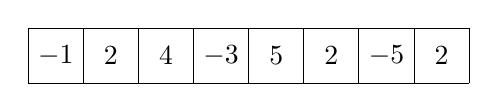
\begin{tikzpicture}[scale=0.7]
\draw (0,0) grid (8,1);

\node at (0.5,0.5) {$-1$};
\node at (1.5,0.5) {$2$};
\node at (2.5,0.5) {$4$};
\node at (3.5,0.5) {$-3$};
\node at (4.5,0.5) {$5$};
\node at (5.5,0.5) {$2$};
\node at (6.5,0.5) {$-5$};
\node at (7.5,0.5) {$2$};
\end{tikzpicture}
\end{center}
\begin{samepage}
\begin{comment}
\end{comment}
the following subarray produces the maximum sum $10$:
\begin{center}
以下の部分列が最大部分列和10を成す。

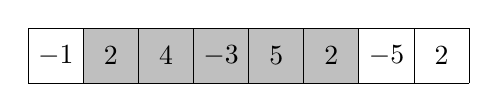
\begin{tikzpicture}[scale=0.7]
\fill[color=lightgray] (1,0) rectangle (6,1);
\draw (0,0) grid (8,1);

\node at (0.5,0.5) {$-1$};
\node at (1.5,0.5) {$2$};
\node at (2.5,0.5) {$4$};
\node at (3.5,0.5) {$-3$};
\node at (4.5,0.5) {$5$};
\node at (5.5,0.5) {$2$};
\node at (6.5,0.5) {$-5$};
\node at (7.5,0.5) {$2$};
\end{tikzpicture}
\end{center}
\end{samepage}

\begin{comment}
We assume that an empty subarray is allowed,
so the maximum subarray sum is always at least $0$.
\end{comment}

ここでは空の部分列も許可される。
そのため、最大の部分列の和は少なくとも0である。

\begin{comment}
\subsubsection{Algorithm 1}

A straightforward way to solve the problem
is to go through all possible subarrays,
calculate the sum of values in each subarray and maintain
the maximum sum.
The following code implements this algorithm:
\end{comment}

\subsubsection{アルゴリズム1}

わかりやすい解法は、部分列を全探索列挙し、それぞれの総和を求め
最大値を保持することである。
このアルゴリズムを実行するとこのようになる:

\begin{lstlisting}
int best = 0;
for (int a = 0; a < n; a++) {
    for (int b = a; b < n; b++) {
        int sum = 0;
        for (int k = a; k <= b; k++) {
            sum += array[k];
        }
        best = max(best,sum);
    }
}
cout << best << "\n";
\end{lstlisting}

\begin{comment}
The variables \texttt{a} and \texttt{b} fix the first and
last index of the subarray,
and the sum of values is calculated to the variable \texttt{sum}.
The variable \texttt{best} contains the maximum sum found during the search.

The time complexity of the algorithm is $O(n^3)$,
because it consists of three nested loops 
that go through the input.
\end{comment}

変数\texttt{a}と\texttt{b}は部分列の先頭と末尾の位置を保持する。
そしてその和が変数\texttt{sum}に格納される。
変数\texttt{best}は探索中に見つけた和の最大値を保持する。

このアルゴリズムは入力に対し三重ネストのループを含んでおり、
時間計算量は$O(n^3)$である。

\begin{comment}
\subsubsection{Algorithm 2}

It is easy to make Algorithm 1 more efficient
by removing one loop from it.
This is possible by calculating the sum at the same
time when the right end of the subarray moves.
The result is the following code:

\begin{lstlisting}
int best = 0;
for (int a = 0; a < n; a++) {
    int sum = 0;
    for (int b = a; b < n; b++) {
        sum += array[b];
        best = max(best,sum);
    }
}
cout << best << "\n";
\end{lstlisting}
\end{comment}

\subsubsection{アルゴリズム 2}

アルゴリズム1の効率を改善する簡単な手法はループを取り除くことである。
部分列の末尾を動かす際、同時に部分列の和を計算していけば
ループを1つ減らすことができる。
その時のコードはこのようになる:

\begin{lstlisting}
int best = 0;
for (int a = 0; a < n; a++) {
    int sum = 0;
    for (int b = a; b < n; b++) {
        sum += array[b];
        best = max(best,sum);
    }
}
cout << best << "\n";
\end{lstlisting}

\begin{comment}
After this change, the time complexity is $O(n^2)$.
\end{comment}

変更後の時間計算量は$O(n^2)$である。

\begin{comment}
\subsubsection{Algorithm 3}

Surprisingly, it is possible to solve the problem
in $O(n)$ time\footnote{In \cite{ben86}, this linear-time algorithm
is attributed to J. B. Kadane, and the algorithm is sometimes
called \index{Kadane's algorithm} \key{Kadane's algorithm}.}, which means
that just one loop is enough.
The idea is to calculate, for each array position,
the maximum sum of a subarray that ends at that position.
After this, the answer for the problem is the
maximum of those sums.

Consider the subproblem of finding the maximum-sum subarray
that ends at position $k$.
There are two possibilities:
\begin{enumerate}
\item The subarray only contains the element at position $k$.
\item The subarray consists of a subarray that ends
at position $k-1$, followed by the element at position $k$.
\end{enumerate}
\end{comment}

\subsubsection{アルゴリズム3}

驚くべきことに、この問題は$O(n)$時間\footnote{\cite{ben86}において
この定数時間アルゴリズムはJ. B. Kadaneによって紹介されたため、
しばしば\index{Kadane's algorithm} \key{Kadane's algorithm}と呼ばれる}、
すなわち単一ループのアルゴリズムで解くことができる。
その基本的なアイデアは、部分列の末尾を探索していく過程で、
その末尾に対応した最大部分和を適宜求めていくことである。

部分列の末尾の位置$k$が固定されている場合に
部分和が最大となる部分列を見つけるという部分問題を考えよう。
そのような部分列には2つの可能性がある:
\begin{enumerate}
\item 部分列は$k$番目の要素のみ含む。
\item 部分列は$k-1$番目の要素を末尾とする部分列に$k$番目の要素を加えたものである。
\end{enumerate}

\begin{comment}
In the latter case, since we want to
find a subarray with maximum sum,
the subarray that ends at position $k-1$
should also have the maximum sum.
Thus, we can solve the problem efficiently
by calculating the maximum subarray sum
for each ending position from left to right.

The following code implements the algorithm:
\end{comment}

後者のケースで考えると、我々は部分列の最大和を求めたいので、
$k-1$番目を末尾とする部分列としては、
そのような部分列のうち最大和となるものを用いたい。
よって、この問題は末尾の位置を左から右に動かしつつ
最大部分列和を適宜求めていくことで効率的に解くことができる。

このアルゴリズムを実装するとこのようになる:

\begin{lstlisting}
int best = 0, sum = 0;
for (int k = 0; k < n; k++) {
    sum = max(array[k],sum+array[k]);
    best = max(best,sum);
}
cout << best << "\n";
\end{lstlisting}

\begin{comment}
The algorithm only contains one loop
that goes through the input,
so the time complexity is $O(n)$.
This is also the best possible time complexity,
because any algorithm for the problem
has to examine all array elements at least once.
\end{comment}

このアルゴリズムは入力データを探索する単一ループしか
持たないため、時間計算量は$O(n)$である。
これは考えうる最良の時間計算量である。
なぜならこの問題を解くうえでいかなるアルゴリズムでも
各要素を最低1回は辿らないといけないためである。

\begin{comment}
\subsubsection{Efficiency comparison}

It is interesting to study how efficient 
algorithms are in practice.
The following table shows the running times
of the above algorithms for different
values of $n$ on a modern computer.

In each test, the input was generated randomly.
The time needed for reading the input was not
measured.

\begin{center}
\begin{tabular}{rrrr}
array size $n$ & Algorithm 1 & Algorithm 2 & Algorithm 3 \\
\hline
$10^2$ & $0.0$ s & $0.0$ s & $0.0$ s \\
$10^3$ & $0.1$ s & $0.0$ s & $0.0$ s \\
$10^4$ & > $10.0$ s & $0.1$ s & $0.0$ s \\
$10^5$ & > $10.0$ s & $5.3$ s & $0.0$ s \\
$10^6$ & > $10.0$ s & > $10.0$ s & $0.0$ s \\
$10^7$ & > $10.0$ s & > $10.0$ s & $0.0$ s \\
\end{tabular}
\end{center}
\end{comment}

\subsubsection{効率の比較}

実際これらのアルゴリズムがどの程度実用的か興味深いことだろう。
下記の表は異なる入力サイズに対する実行時間を示している。

各実験において、入力はランダムに生成された。
また入力を読み込む時間は含んでいない。

\begin{center}
\begin{tabular}{rrrr}
入力サイズ $n$ & アルゴリズム1 & アルゴリズム2 & アルゴリズム3 \\
\hline
$10^2$ & $0.0$ s & $0.0$ s & $0.0$ s \\
$10^3$ & $0.1$ s & $0.0$ s & $0.0$ s \\
$10^4$ & > $10.0$ s & $0.1$ s & $0.0$ s \\
$10^5$ & > $10.0$ s & $5.3$ s & $0.0$ s \\
$10^6$ & > $10.0$ s & > $10.0$ s & $0.0$ s \\
$10^7$ & > $10.0$ s & > $10.0$ s & $0.0$ s \\
\end{tabular}
\end{center}

\begin{comment}
The comparison shows that all algorithms
are efficient when the input size is small,
but larger inputs bring out remarkable
differences in the running times of the algorithms.
Algorithm 1 becomes slow
when $n=10^4$, and Algorithm 2
becomes slow when $n=10^5$.
Only Algorithm 3 is able to process
even the largest inputs instantly.
\end{comment}

この比較より、入力サイズが小さい場合はどのアルゴリズムも十分高速であるが、
入力サイズが大きくなると大きな差が生じることがわかる。
アルゴリズム1は$n=10^4$、アルゴリズム2は$n=10^5$ごろから
遅くなるが、アルゴリズム3は大きな入力サイズでも
十分に対応できる。
